
%(BEGIN_QUESTION)
% Copyright 2006, Tony R. Kuphaldt, released under the Creative Commons Attribution License (v 1.0)
% This means you may do almost anything with this work of mine, so long as you give me proper credit

Differansetrykktransmittere er svært vanlige i prosessindustri.  I tillegg til trykkmåling kan de brukes til å inferere nivå, flow og tetthet.  En standard manifold kalt en \textit{treventilsmanifold} brukes ofte mellom prosess og transmitter.  Den består av to block-ventiler (isolering av ``high'' og ``low'' port) og én ``equalizing''-ventil (kobler sidene sammen for null differansetrykk).

Treventilsmanifolder leveres ofte som én enhet, men kan også bygges av tre separate ventiler, to T-koblinger og nødvendige koblinger til transmitter.

\vskip 10pt

Anta en differansetrykktransmitter som måler trykkfall over en varmeveksler.  Typisk trykk oppstrøms er 1000 PSI og nedstrøms 970 PSI.  Transmitteren er koblet via treventilsmanifold.  En enkel ``bleed''-ventil på lavtrykksiden brukes for avlufting før demontering:

$$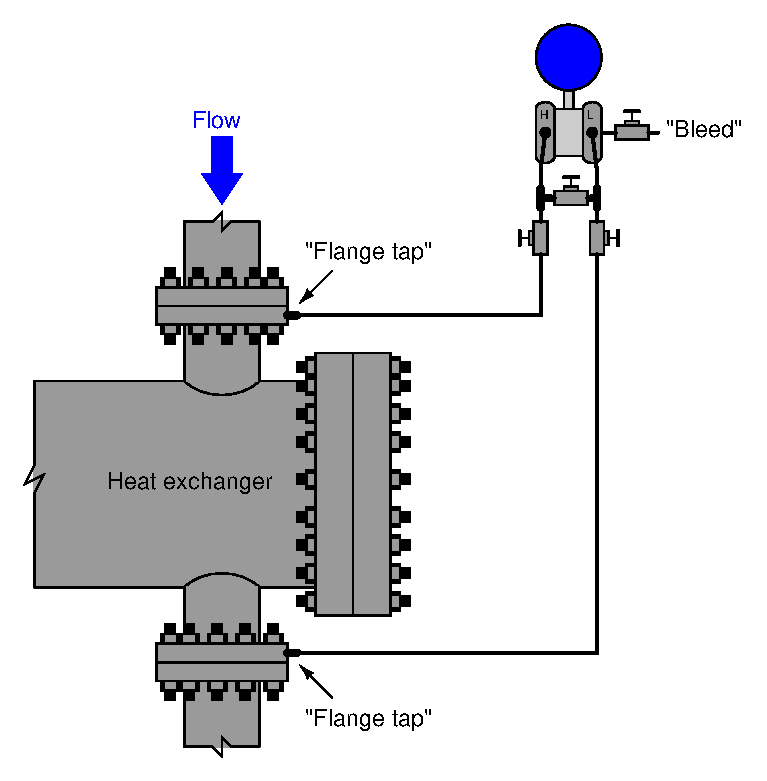
\includegraphics[width=15.5cm]{i00211x01.eps}$$

Vanlig prosedyre for uttak fra drift er: lukk high-side block, åpne equalizing, lukk low-side block.  Når transmitteren er isolert og differansetrykket utjevnet, åpnes bleed forsiktig for å avlaste lagret trykk til atmosfære.

Bestem trykket på hver side av transmitteren i hvert steg:

% No blank lines allowed between lines of an \halign structure!
% I use comments (%) instead, so that TeX doesn't choke.

$$\vbox{\offinterlineskip
\halign{\strut
\vrule \quad\hfil # \ \hfil & 
\vrule \quad\hfil # \ \hfil & 
\vrule \quad\hfil # \ \hfil & 
\vrule \quad\hfil # \ \hfil \vrule \cr
\noalign{\hrule}
%
% First row
Step & High-side pressure & Low-side pressure & Differential pressure \cr
%
\noalign{\hrule}
%
% Another row
Transmitter in service & 1000 PSI & 970 PSI & 30 PSID \cr
%
\noalign{\hrule}
%
% Another row
Close high-side block valve &  &  &  \cr
%
\noalign{\hrule}
%
% Another row
Open equalizing valve &  &  &  \cr
%
\noalign{\hrule}
%
% Another row
Close low-side block valve &  &  &  \cr
%
\noalign{\hrule}
%
% Another row
Open bleed valve &  &  &  \cr
%
\noalign{\hrule}
} % End of \halign 
}$$ % End of \vbox

Anta nå alternativ rekkefølge ved senere anledning: lukk low-side block først, så equalize, så blokk high side.

Bestem trykkene gjennom denne alternative prosedyren:

% No blank lines allowed between lines of an \halign structure!
% I use comments (%) instead, so that TeX doesn't choke.

$$\vbox{\offinterlineskip
\halign{\strut
\vrule \quad\hfil # \ \hfil & 
\vrule \quad\hfil # \ \hfil & 
\vrule \quad\hfil # \ \hfil & 
\vrule \quad\hfil # \ \hfil \vrule \cr
\noalign{\hrule}
%
% First row
Step & High-side pressure & Low-side pressure & Differential pressure \cr
%
\noalign{\hrule}
%
% Another row
Transmitter in service & 1000 PSI & 970 PSI & 30 PSID \cr
%
\noalign{\hrule}
%
% Another row
Close low-side block valve &  &  &  \cr
%
\noalign{\hrule}
%
% Another row
Open equalizing valve &  &  &  \cr
%
\noalign{\hrule}
%
% Another row
Close high-side block valve &  &  &  \cr
%
\noalign{\hrule}
%
% Another row
Open bleed valve &  &  &  \cr
%
\noalign{\hrule}
} % End of \halign 
}$$ % End of \vbox

Basert på transmittertrykk i begge prosedyrer: anbefaler du den ene fremfor den andre?  Hvorfor?

\vskip 20pt \vbox{\hrule \hbox{\strut \vrule{} {\bf Suggestions for Socratic discussion} \vrule} \hrule}

\begin{itemize}
\item{} Et nyttig problemløsningsverktøy er tankeeksperiment: simuler systemrespons mentalt under gitte betingelser.  Forklar hvordan dette er nyttig for å vurdere sikreste treventilsprosedyre.
\end{itemize}

\underbar{file i00211}
%(END_QUESTION)





%(BEGIN_ANSWER)


%(END_ANSWER)





%(BEGIN_NOTES)

Ved prosedyren ``HEL'' (High, Equalize, Low):

% No blank lines allowed between lines of an \halign structure!
% I use comments (%) instead, so that TeX doesn't choke.

$$\vbox{\offinterlineskip
\halign{\strut
\vrule \quad\hfil # \ \hfil & 
\vrule \quad\hfil # \ \hfil & 
\vrule \quad\hfil # \ \hfil & 
\vrule \quad\hfil # \ \hfil \vrule \cr
\noalign{\hrule}
%
% First row
Step & High-side pressure & Low-side pressure & Differential pressure \cr
%
\noalign{\hrule}
%
% Another row
Transmitter in service & 1000 PSI & 970 PSI & 30 PSID \cr
%
\noalign{\hrule}
%
% Another row
Close high-side block valve & 1000 PSI & 970 PSI & 30 PSID \cr
%
\noalign{\hrule}
%
% Another row
Open equalizing valve & 970 PSI & 970 PSI & 0 PSID \cr
%
\noalign{\hrule}
%
% Another row
Close low-side block valve & 970 PSI & 970 PSI & 0 PSID \cr
%
\noalign{\hrule}
%
% Another row
Open bleed valve & 0 PSI & 0 PSI & 0 PSID \cr
%
\noalign{\hrule}
} % End of \halign 
}$$ % End of \vbox

\vskip 10pt

Ved prosedyren ``LEH'' (Low, Equalize, High):

% No blank lines allowed between lines of an \halign structure!
% I use comments (%) instead, so that TeX doesn't choke.

$$\vbox{\offinterlineskip
\halign{\strut
\vrule \quad\hfil # \ \hfil & 
\vrule \quad\hfil # \ \hfil & 
\vrule \quad\hfil # \ \hfil & 
\vrule \quad\hfil # \ \hfil \vrule \cr
\noalign{\hrule}
%
% First row
Step & High-side pressure & Low-side pressure & Differential pressure \cr
%
\noalign{\hrule}
%
% Another row
Transmitter in service & 1000 PSI & 970 PSI & 30 PSID \cr
%
\noalign{\hrule}
%
% Another row
Close low-side block valve & 1000 PSI & 970 PSI & 30 PSID \cr
%
\noalign{\hrule}
%
% Another row
Open equalizing valve & 1000 PSI & 1000 PSI & 0 PSID \cr
%
\noalign{\hrule}
%
% Another row
Close high-side block valve & 1000 PSI & 1000 PSI & 0 PSID \cr
%
\noalign{\hrule}
%
% Another row
Open bleed valve & 0 PSI & 0 PSI & 0 PSID \cr
%
\noalign{\hrule}
} % End of \halign 
}$$ % End of \vbox

\vskip 10pt

HEL-prosedyren gir mindre trykk som må avluftes til atmosfære enn LEH-prosedyren.  I dette eksemplet er forskjellen liten, men ved større normale differansetrykk blir forskjellen mer betydelig.  HEL er derfor å foretrekke.

%INDEX% Process: heat exchanger pressure drop measurement (generic)
%INDEX% Safety, isolation valves: 3-valve equalizing manifold

%(END_NOTES)

